\tectcolor{principal}{Metodo With-and-Without}\\

Los \textcolor{principal}{Métodos de Valor Diferencial (``DVM'')} son estrategias de valuación pertenecientes al enfoque de ingresos, las cuales estiman el valor de un activo a través de una comparativa entre el valor del negocio \textbf{CON} la inclusión del activo y el valor del negocio \textbf{SIN} la presencia del activo. Estos métodos son especialmente utilizados en la valoración de aquellos activos para los que es complicado asignar directamente un flujo de ingresos, pese a que son vitales en la generación de dichos ingresos. Los \textcolor{principal}{DVM} generalmente se implementan en dos modalidades: \textcolor{principal}{el \textit{Método With-and-Without} y el Método \textit{Greenfield.}}\\

%El Método \textcolor{principal}{\textit{With-and-Without}}, se enfoca en el cálculo del valor del activo intangible en análisis mediante la probabilidad ponderada de la diferencia en el valor del negocio, estimada bajo dos distintos flujos de efectivo proyectados:
%
%\begin{enumerate}[H] 
%\item  El valor del negocio con todos los activos 
%\item  El valor del negocio con todos los activos, \textbf{EXCEPTUANDO} el activo intangible objeto de valoración.
%\end{enumerate}

\begin{figure}[H]
\centering
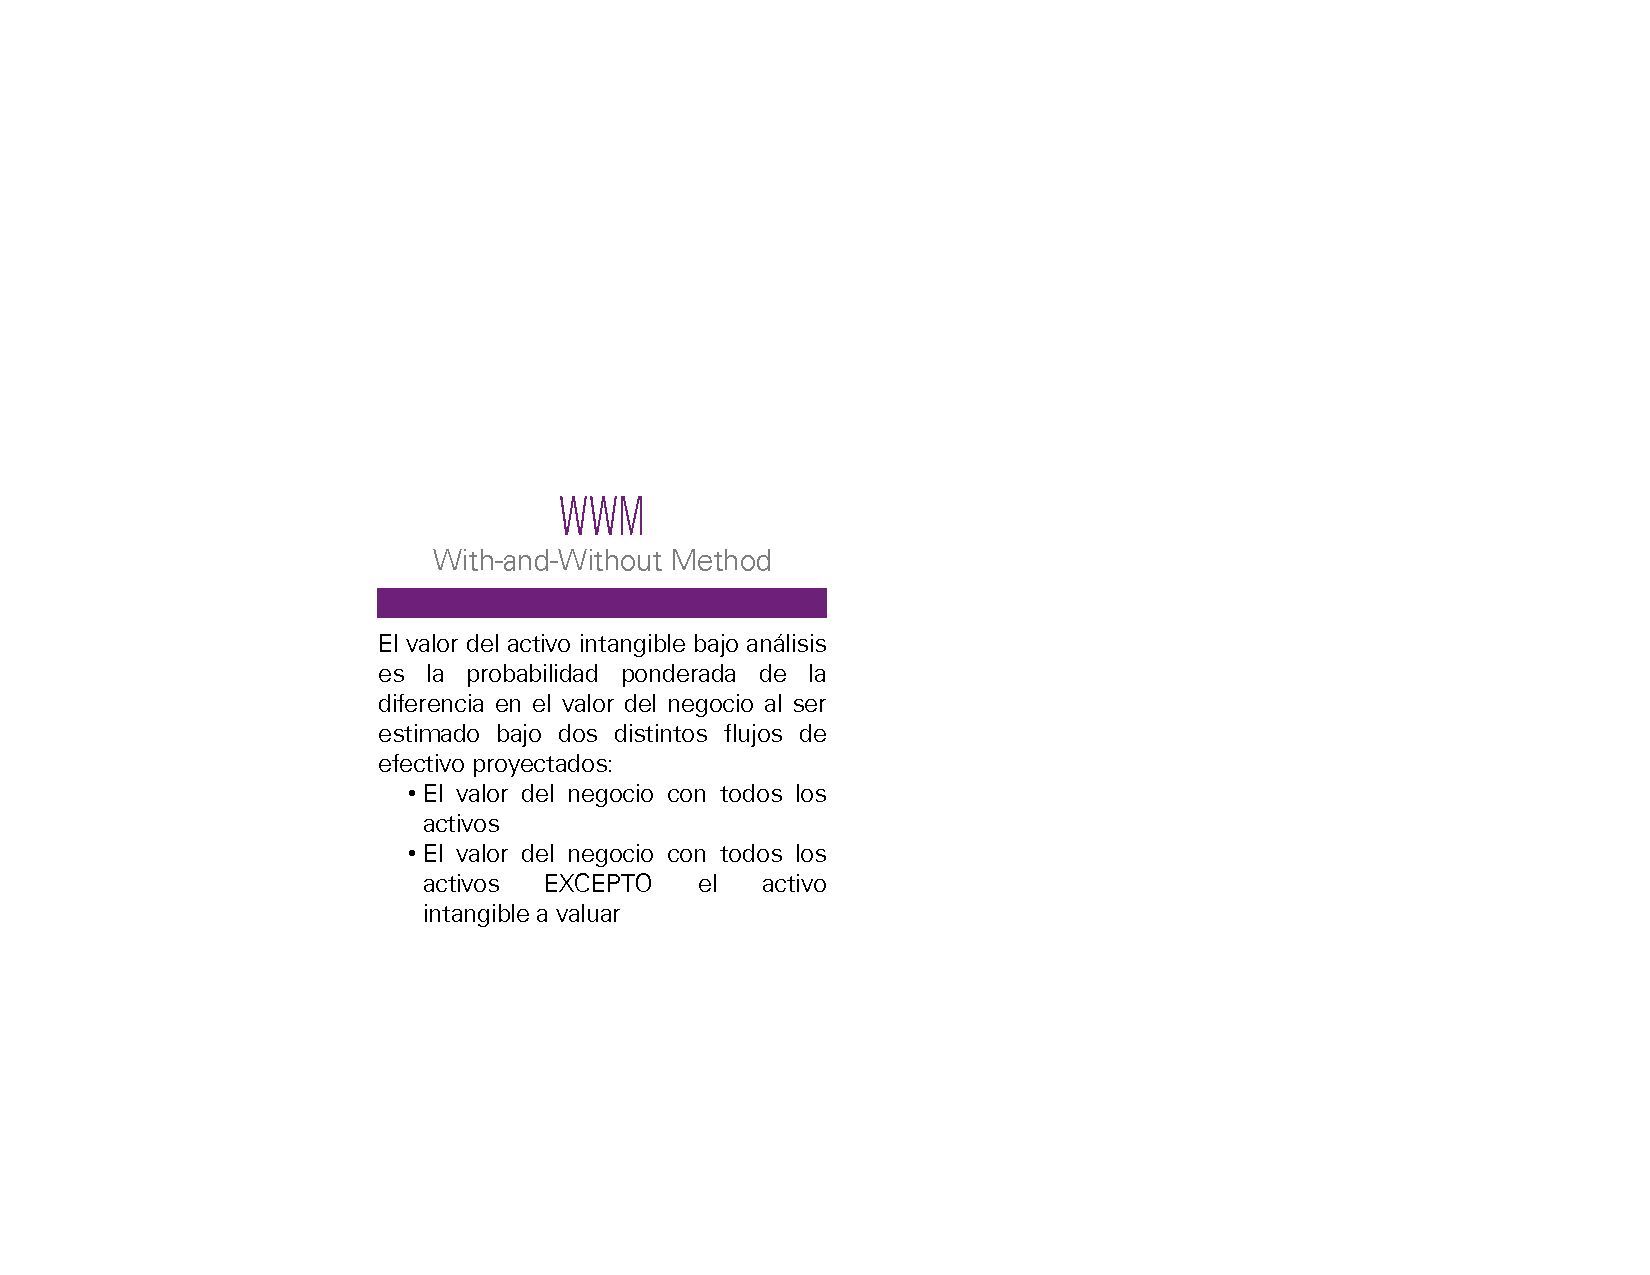
\includegraphics[width=.5\textwidth]{\rutaImagenes/wwm}
\end{figure}


Este método ha probado ser efectivo en la valoración de ciertos tipos de activos, tales como \textcolor{principal}{licencias de transmisión y franquicias}. Para su correcta implementación, es crucial contar con proyecciones precisas de los ingresos y gastos del negocio durante el período de análisis.\\

El método \textit{With-and-Without} posee ciertas ventajas y desventajas. Entre las ventajas, destaca su utilidad en la valoración de activos que, si bien no son los principales generadores de ingresos del negocio, sí contribuyen a su generación. Además, este método no requiere calcular cargos por activos.\\

En cuanto a las desventajas, se debe tener en cuenta que la calidad del análisis depende en gran medida de la exactitud de los supuestos asumidos. Asimismo, se supone que los activos comprados o construidos sólo generan utilidades en relación con su costo, lo cual puede no ser preciso en todas las circunstancias.\\

